\tikzset{%
   neuron missing/.style={
    draw=none, 
    scale=4,
    text height=0.333cm,
    execute at begin node=\color{black}$\vdots$
  },
}

\begin{figure}[H]
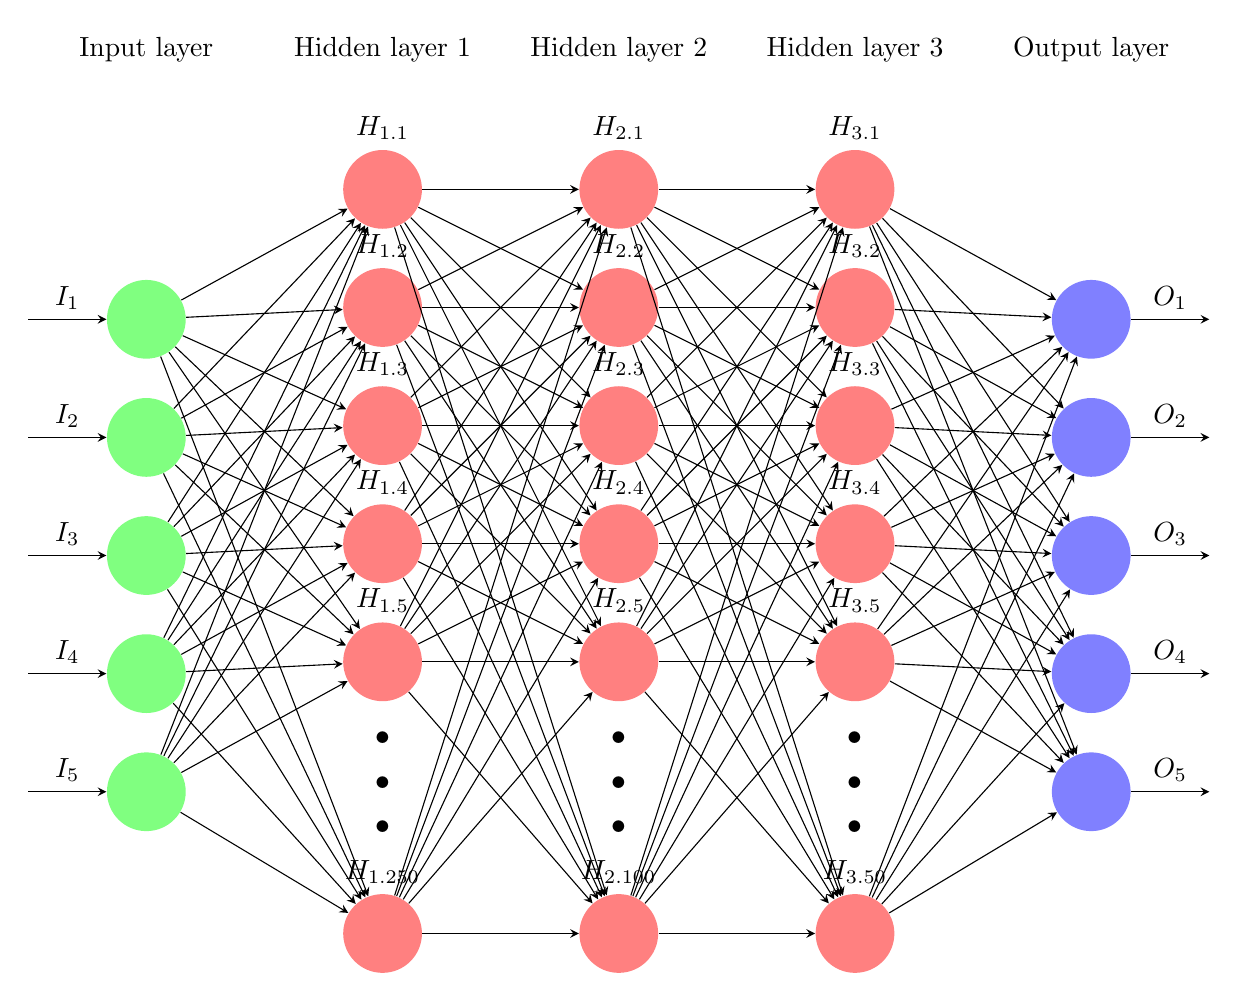
\begin{tikzpicture}[x=1.5cm, y=1.5cm, >=stealth]
%=========================================================================================================
% Input layer
%=========================================================================================================

%First 3 nodes drawn in input layer
\foreach \m/\l [count=\y] in {1,...,5}
{
 \node [circle,fill=green!50,minimum size=1cm] (input-\m) at (0,0.9-\y) {};
}

%Name the input node with 1-256 with the I_1 - I_256, with the arrow coming in
\foreach \l [count=\i] in {1,...,5}
  \draw [<-] (input-\i) -- ++(-1,0)
    node [above, midway] {$I_{\l}$};

%=========================================================================================================
% Hidden layer - 1
%=========================================================================================================
 
%First node drawn in hidden layer
\foreach \m [count=\y] in {1,...,5}
  \node [circle,fill=red!50,minimum size=1cm ] (hidden1-\m) at (2,2-\y) {};
  
% %Last node drawn in hidden layer
 \foreach \m [count=\y] in {6}
   \node [circle,fill=red!50,minimum size=1cm ] (hidden1-\m) at (2,-4.3-\y) {};

%3 dots marked in hidden layer  
 \node [neuron missing]  at (2,-4) {};

% %Name the hidden layer nodes 1-16 as H_1 - H16 above the node
 \foreach \l [count=\i] in {1,...,5,250}
   \node [above] at (hidden1-\i.north) {$H_{1.\l}$};

%=========================================================================================================
% Hidden layer - 2
%=========================================================================================================

%First node drawn in hidden layer
\foreach \m [count=\y] in {1,...,5}
  \node [circle,fill=red!50,minimum size=1cm ] (hidden2-\m) at (4,2-\y) {};
  
% %Last node drawn in hidden layer
 \foreach \m [count=\y] in {6}
   \node [circle,fill=red!50,minimum size=1cm ] (hidden2-\m) at (4,-4.3-\y) {};

%3 dots marked in hidden layer  
 \node [neuron missing]  at (4,-4) {};

% %Name the hidden layer nodes 1-16 as H_1 - H16 above the node
 \foreach \l [count=\i] in {1,...,5,100}
   \node [above] at (hidden2-\i.north) {$H_{2.\l}$};
   
%=========================================================================================================
% Hidden layer - 3
%=========================================================================================================

%First node drawn in hidden layer
\foreach \m [count=\y] in {1,...,5}
  \node [circle,fill=red!50,minimum size=1cm ] (hidden3-\m) at (6,2-\y) {};
  
% %Last node drawn in hidden layer
 \foreach \m [count=\y] in {6}
   \node [circle,fill=red!50,minimum size=1cm ] (hidden3-\m) at (6,-4.3-\y) {};

%3 dots marked in hidden layer  
 \node [neuron missing]  at (6,-4) {};

% %Name the hidden layer nodes 1-16 as H_1 - H16 above the node
 \foreach \l [count=\i] in {1,...,5,50}
   \node [above] at (hidden3-\i.north) {$H_{3.\l}$};   

   
%=========================================================================================================
% Output layer
%=========================================================================================================

%First node drawn in output layer
%\foreach \m [count=\y] in {1}
%  \node [circle,fill=blue!50,minimum size=1cm ] (output-\m) at (8,-1-\y) {};

%Name the output layer nodes 1-16 as O_1 - O_16 with the arrows going out
%\foreach \l [count=\i] in {1}
%  \draw [->] (output-\i) -- ++(1,0)
%    node [above, midway] {$O_{ \l}$};

\foreach \m [count=\y] in {1,...,5}
  \node [circle,fill=blue!50,minimum size=1cm ] (output-\m) at (8,0.9-\y) {};
  
\foreach \l [count=\i] in {1,...,5}
  \draw [->] (output-\i) -- ++(1,0)
    node [above, midway] at (output-\i.north) {$O_{\l}$}; 

%=========================================================================================================
% Draw connections
%=========================================================================================================
%Connections between input layer and hidden layer
\foreach \i in {1,...,5}
  \foreach \j in {1,...,6}
    \draw [->] (input-\i) -- (hidden1-\j);
    
\foreach \i in {1,...,6}
  \foreach \j in {1,...,6}
    \draw [->] (hidden1-\i) -- (hidden2-\j);

\foreach \i in {1,...,6}
  \foreach \j in {1,...,6}
    \draw [->] (hidden2-\i) -- (hidden3-\j);    
    
%\foreach \i in {1,...,6}
%  \foreach \j in {1,...,1}
%    \draw [->] (hidden2-\i) -- (hidden3-\j);

%Connections between hidden layer and output layer
\foreach \i in {1,...,6}
  \foreach \j in {1,...,5}
    \draw [->] (hidden3-\i) -- (output-\j);

%=========================================================================================================
% Draw headers
%=========================================================================================================
%headers
\foreach \l [count=\x from 0] in {Input layer, Hidden layer 1, Hidden layer 2, Hidden layer 3, Output layer}
  \node [align=center, above] at (\x*2,2) {\l};

\end{tikzpicture}
\caption{Visualisation of the model}
\end{figure}